\documentclass[10pt]{beamer}
\usepackage{etex}
\usepackage[T1]{fontenc}
\usepackage[bitstream-charter]{mathdesign}
\usepackage[scaled=0.92]{PTSans}
\renewcommand*\ttdefault{lmvtt}
\usepackage{exscale}

\usepackage[final,expansion=alltext]{microtype}
\usepackage[english]{babel}
\usepackage{ragged2e}

\usepackage{amsmath}
\usepackage{graphicx}                               % graphics
\usepackage{booktabs, array}                        % nice tables
\usepackage[algoruled]{algorithm2e}                 % pseudocode
\usepackage[numbers,sort]{natbib}                   % better bibliography
\usepackage{cleveref}                               % the best package ever
\usepackage[acronym,smallcaps,nowarn]{glossaries}   % second best package ever

% COLORS
\newcommand{\gray}[1]{\textcolor{black!60}{#1}}
\newcommand{\blu}[1]{\textcolor{jblue}{#1}}

\newacronym{ELBO}{elbo}{evidence lower bound}
\newacronym{KL}{kl}{Kullback-Leibler}

\newacronym{DEF}{def}{deep exponential family}
\newacronym{DLGM}{dlgm}{deep latent Gaussian model}
\newacronym{DRAW}{draw}{Deep Recurrent Attentive Writer}

\newacronym{MF}{mf}{mean-field}
\newacronym{VGP}{vgp}{variational Gaussian process}
\newacronym{BBVI}{bbvi}{black box variational inference}
\newacronym{ADVI}{advi}{automatic differentiation variational inference}
\newacronym{NF}{nf}{normalizing flows}
\newacronym{CVI}{cvi}{copula variational inference}
\newacronym{VAE}{vae}{variational autoencoder}
\newacronym{IWAE}{iwae}{importance weighted autoencoder}
\newacronym{NVIL}{nvil}{neural variational inference}
\newacronym{MIXTURE}{mixture}{}
\newacronym{DSVI}{dsvi}{}

\newacronym{VI}{vi}{variational inference}
\newacronym{EP}{ep}{expectation propagation}

\newacronym{LS}{ls}{Langevin-Stein}
\newacronym{OPVI}{opvi}{operator variational inference}

\DeclareRobustCommand{\mb}[1]{\ensuremath{\boldsymbol{\mathbf{#1}}}}
\DeclareRobustCommand{\mbf}[1]{\ensuremath{\textbf{#1}}}
\DeclareMathOperator*{\argmax}{arg\,max}
\DeclareMathOperator*{\argmin}{arg\,min}


\newcommand{\KL}[2]{\ensuremath{\textrm{KL}\left(#1\;\|\;#2\right)}}

\renewcommand{\mid}{~\vert~}

\newcommand{\mbw}{\mb{w}}
\newcommand{\mbW}{\mb{W}}

\newcommand{\mbx}{\mb{x}}
\newcommand{\mbX}{\mbf{X}}

\newcommand{\mby}{\mb{y}}
\newcommand{\mbY}{\mbf{Y}}

\newcommand{\mbz}{\mb{z}}
\newcommand{\mbZ}{\mb{Z}}

\newcommand{\mbI}{\mbf{I}}
\newcommand{\mbone}{\mbf{1}}

\newcommand{\mbL}{\mbf{L}}

\newcommand{\mbtheta}{\mb{\theta}}
\newcommand{\mbTheta}{\mb{\Theta}}
\newcommand{\mbomega}{\mb{\omega}}
\newcommand{\mbOmega}{\mb{\Omega}}
\newcommand{\mbsigma}{\mb{\sigma}}
\newcommand{\mbSigma}{\mb{\Sigma}}
\newcommand{\mbphi}{\mb{\phi}}
\newcommand{\mbPhi}{\boldsymbol{\Phi}}
% \newcommand{\mblambda}{\mb{\lambda}}

\newcommand{\mbalpha}{\mb{\alpha}}
\newcommand{\mbbeta}{\mb{\beta}}
\newcommand{\mbgamma}{\mb{\gamma}}
\newcommand{\mbeta}{\mb{\eta}}
\newcommand{\mbmu}{\mb{\mu}}
\newcommand{\mbrho}{\mb{\rho}}
\newcommand{\mblambda}{\mb{\lambda}}
\newcommand{\mbzeta}{\mb{\zeta}}

\newcommand\dif{\mathop{}\!\mathrm{d}}
\newcommand{\diag}{\textrm{diag}}
\newcommand{\supp}{\textrm{supp}}

\newcommand{\E}{\mathbb{E}}
\newcommand{\bbH}{\mathbb{H}}
\newcommand{\Var}{\mathbb{V}\textrm{ar}}

\newcommand{\bbN}{\mathbb{N}}
\newcommand{\bbZ}{\mathbb{Z}}
\newcommand{\bbR}{\mathbb{R}}
\newcommand{\bbS}{\mathbb{S}}

\newcommand{\cL}{\mathcal{L}}

\newcommand{\cN}{\mathcal{N}}
\newcommand{\cT}{\mathcal{T}}
\newcommand{\Gam}{\textrm{Gam}}
\newcommand{\InvGam}{\textrm{InvGam}}

\usepackage{tikz}
\usetikzlibrary{bayesnet}

\pgfdeclarelayer{edgelayer}
\pgfdeclarelayer{nodelayer}
\pgfsetlayers{edgelayer,nodelayer,main}

\definecolor{hexcolor0xbfbfbf}{rgb}{0.749,0.749,0.749}

\tikzset{>=latex}
\tikzstyle{none}   = [inner sep=0pt]
\tikzstyle{line}   = [-,
                      thick,
                      shorten <=1pt,
                      shorten >=1pt]
\tikzstyle{arrow}  = [->,
                      thick,
                      shorten <=1pt,
                      shorten >=1pt]
\tikzstyle{ardash} = [dashed,
                      ->,
                      thick,
                      shorten <=1pt,
                      shorten >=1pt]

\tikzstyle{empty}=[
                   circle,
                   opacity=0.0,
                   text opacity=1.0,
                   inner sep=0pt
                  ]

\tikzstyle{box}=[
                 rectangle,
                 fill=White,
                 thick,
                 draw=Black,
                 inner sep=7pt
                ]

\tikzstyle{filled}=[
                    circle,
                    thick,
                    fill=hexcolor0xbfbfbf,
                    draw=Black
                   ]

\tikzstyle{hollow}=[
                    circle,
                    thick,
                    fill=White,
                    draw=Black
                   ]

\tikzstyle{param}=[
                   rectangle,
                   fill=Black,
                   draw=Black,
                   inner sep=0pt,
                   minimum width=4pt,
                   minimum height=4pt
                  ]

\tikzstyle{paramhollow}=[
                         rectangle,
                         thick,
                         fill=White,
                         draw=Black,
                         inner sep=0pt,
                         minimum
                         width=4pt,
                         minimum height=4pt
                        ]

\usepackage{pgfplots}                               % PGFPLOTS baby!
\pgfplotsset{compat=newest}
\pgfplotsset{plot coordinates/math parser=false}
% \usepgfplotslibrary{statistics}


\usetheme{simple}

\addbibresource{2017-04-Edward.bib}

% Watermark background (simple theme)
% \setwatermark{\includegraphics[height=8cm]{img/Heckert_GNU_white.png}}


\title{Probabilistic programming with Edward}
% \subtitle{}
\date{April 25, 2017}
\author{John Reid}
\institute{Biostatistics Unit, \\ School of Clinical Medicine, \\ Cambridge University}

\begin{document}

\maketitle

\begin{frame}
\frametitle{George E.P. Box (1919 - 2013)}
\begin{columns}
\begin{column}{0.4\textwidth}
    \begin{center}
     \includegraphics[width=\columnwidth]{img/box.jpg}
     \end{center}
\end{column}
\begin{column}{0.6\textwidth}
An iterative process for science:
\\[1ex]
\begin{enumerate}
\item Build a model of the science
\\[1ex]
\item Infer the model given data
\\[1ex]
\item Criticize the model given data
\end{enumerate}
\end{column}
\end{columns}
\cite{box_useful_1962-1, box_experimental_1965-1, box_discrimination_1967-1, box_science_1976-1, box_sampling_1980-1}
\end{frame}

\begin{frame}
\frametitle{Box's Loop}
\center
\begin{tikzpicture}[remember picture]
  \node [block] (Infer) {Infer};
  \coordinate[below of=Infer] (under);
  \node [block, left=of Infer] (Model) {Model};
  \draw [->, thick] (Model) -- (Infer);
  \node [block, right=of Infer] (Criticise) {Criticise};
  \draw [->, thick] (Infer) -- (Criticise);
  \draw [->, thick, rounded corners] (Criticise) -- (under) -- (Model);
  \node [block, above=of Infer, fill=blue!20] (Data) {Data};
  \draw [->, thick] (Data) -- (Infer);
\end{tikzpicture} \\
\vspace{20pt}
Edward is a library designed around this loop. \\
\citep{box_science_1976-1, box_sampling_1980-1, david_m._blei_build_2014}
\end{frame}


\begin{frame}
\vspace{3ex}
\textbf{Edward} is a probabilistic programming language,
designed for fast experimentation and research~\citep{tran_deep_2017}.

\emph{Modelling}
\begin{itemize}
\item Composable Turing-complete language of random variables.
\item Examples: Graphical models, neural networks, probabilistic programs.
\item Many data types, tensor vectorization, broadcasting, 3rd party support.
\end{itemize}

\emph{Inference}
\begin{itemize}
\item Composable language for hybrids, message passing, data subsampling.
\item Examples: Black box VI, Hamiltonian MC, stochastic gradient MCMC,
  generative adversarial networks.
\item Infrastructure to develop your own algorithms.
\end{itemize}

\emph{Criticism}
\begin{itemize}
\item Examples: Scoring rules, hypothesis tests, predictive checks.
\end{itemize}

\vspace{1ex}
Built on TensorFlow (features distributed computing, GPUs, autodiff).
\end{frame}

\begin{frame}[fragile]
\inputminted{python}{beta-bernoulli.py}
\end{frame}

\begin{frame}[fragile]
  \begin{block}{Model code}
    \begin{minted}{python}
      p = Beta(a=1.0, b=1.0)
      x = Bernoulli(p=tf.ones(10) * p)
    \end{minted}
  \end{block}
  The random variables $p$ and $x$ are represented by tensors $p^*$ and $x^*$ in the tensorflow computation graph
  \begin{block}{Computation graph}
    \begin{center}
      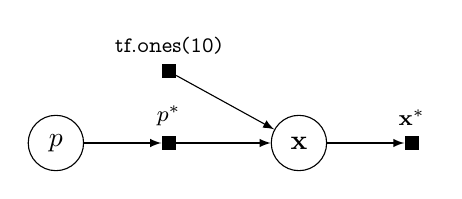
\begin{tikzpicture}[x=1.7cm,y=1.8cm,scale=0.9]
%\begin{tikzpicture}[scale=0.6]

  % Nodes
  \node[latent] (p) {$p$};
  \factor[right=of p, xshift=0.3cm] {thetastar} {$p^*$} {} {};

  \factor[above=of thetastar] {n} {\texttt{tf.ones(10)}} {} {};
  \node[latent, right=of thetastar, xshift=-0.5cm] (x) {$\mbx$};
  \factor[right=of x, xshift=0.3cm] {xstar} {$\mbx^*$} {} {};

  % Edges
  \edge{p}{thetastar};
  \edge{thetastar}{x};
  \edge{n}{x};
  \edge{x}{xstar};

\end{tikzpicture}

    \end{center}
  \end{block}
  Random variables are equipped with methods for likelihoods $\log(x|p)$,
  expectations $\mathbb{E}_{p(x|p)}[x]$, and sampling $\sim p(x|p)$.

  Graph can be executed by \mintinline{python}|x.value()| which returns the tensor $x^*$ and simulates the
  generative process.
\end{frame}

\begin{frame}[fragile]
  Key concept is compositionality:
  \begin{itemize}
    \item Graphs can contain arbitrary tensorflow constructs
    \item Tensorflow conditional evaluations permit construction of nonparametric processes
    \item Graphs can interface with third party tensorflow libraries, e.g. Keras for
      deep learning
  \end{itemize}
  \begin{block}{Deep generative model}
    \begin{minted}{python}
      from edward.models import Bernoulli, Normal
      from keras.layers import Dense

      z = Normal(mu=tf.zeros([N, d]), sigma=tf.ones([N, d]))
      h = Dense(256, activation='relu')(z.value())
      x = Bernoulli(logits=Dense(28 * 28)(h))
    \end{minted}
  \end{block}
\end{frame}

\begin{frame}[allowframebreaks]%in case more than 1 slide needed
\setbeamertemplate{bibliography item}[text]
\bibliographystyle{apalike}
\renewcommand*{\bibfont}{\small}
\printbibliography
\end{frame}
\end{document}
